\documentclass[12pt]{article}
\usepackage{graphicx}
\usepackage{fullpage}
\usepackage{float}

\title{Writeup - Sorting: Putting Your Affairs in Order}
\author{Lev Teytelman}
\date{\today}

\begin{document}\maketitle
\section{Introduction}
This assignment shows the efficiencies of a number of different sorts. The created program takes command-line flags to specify which sorts to do, the number of elements to create and sort, the number of elements to print, and the seed for the random number generator. It then runs the enabled sorts and prints the number of moves and compares for each one, along with all, some, or none of the sorted array.

This writeup will mainly focus on the trends of comparisons and moves for each sort as the number of elements increases. The sorts were run for $\approx1,000$ iterations per type of sort, going in steps of 1 from 2-10, and subsequently going up in increments of 10 to 10,000. Certain sorts took longer to complete all iterations than others, and we will discuss why that is the case.

\section{Scalability}
For this program, an array of $n$ numbers is required. In order to utilize memory in a smart way and most efficiently, the program uses \verb|memalloc| to specify how much space is being set aside and \verb|free| to make it available to the system after use:
\begin{verbatim}
    uint32_t *arr = (uint32_t *) malloc(size * sizeof(uint32_t));
    // use the array here
    free(arr);
\end{verbatim}
The code also re-uses the array instead of allocating four different ones, so as to use up memory with maximum efficiency. This allows the array to take up almost as much memory as the environment has available without having to worry about sharing.

\section{Moves and Comparisons}
As the number of elements to be sorted increases, the number of moves and comparisons is expected to increase as well. The question, however, is how quickly it increases relative to the number of elements - this is described as O notation, and denotes the efficiency of an algorithm.

When plotting these trends, it is clearly visible that Insertion Sort is many times worse than the others, especially as the array size grows. Notice that both axes are logarithmic, meaning the difference between the values at the ends of the lines is much larger than first appears (over 10 times!). It's also seen that Batcher Sort does less moves than Heap Sort; however, it is a constant difference: the gap becomes smaller as the scale increases. Quick Sort eventually beats out all the sorts in both moves and compares, despite the jaggedness of the line. That brings us to our next point: Quick Sort's outputs are unusually varied, especially when compared to the other sorts. This is because our Quick Sort algorithm is unstable: the ``pivot element" around which the other elements are sorted is chosen essentially randomly, and can be an average number, with a balanced recursive sort, or an outlier, causing one side to have many more elements than the other and therefore taking more iterations to sort. This is why Quick Sort has a best case scenario of $O(n\log(n))$, and a worst case of $O(n^2)$, and the reason for the inconsistency.


% [H] to position from:
% https://stackoverflow.com/questions/4294142/how-can-i-position-a-figure-in-latex
\begin{figure}[H]\begin{centering}
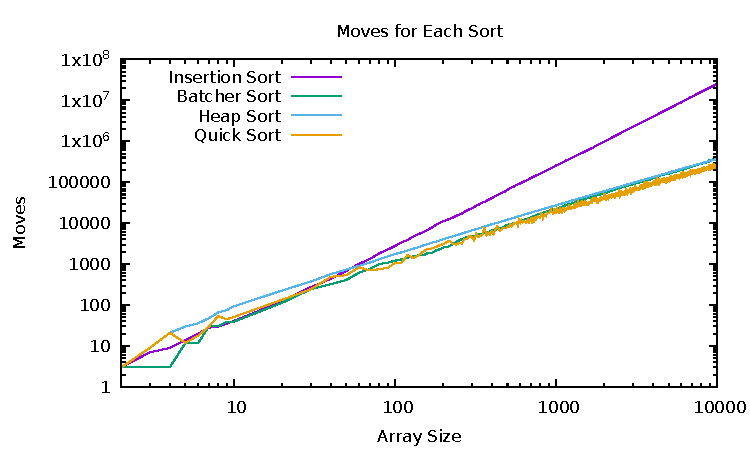
\includegraphics{plots/moves.pdf}\caption{The number of moves needed to sort an array with $x$ elements}
\end{centering}\end{figure}

The graph of compares tells a similar story: Insertion Sort is much less efficient than the others. However, the difference between the number of compares for Batcher and Heap Sorts seems to be growing as the numbers grow; the gap expands, even on the logarithmic scale, representing the O notation's constant $c$. Quick Sort has a similarly jagged line, though a smaller range of compares (the variance is smaller than the variance in the number of moves).

\begin{figure}[H]\begin{centering}
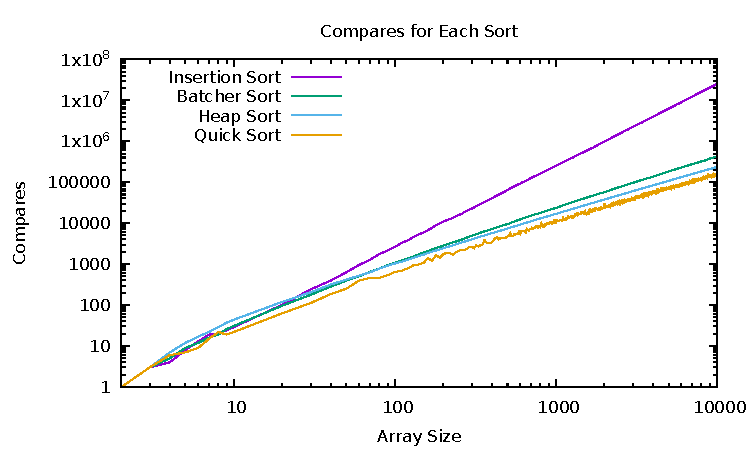
\includegraphics{plots/compares.pdf}\caption{The number of comparisons needed to sort an array with $x$ elements}
\end{centering}\end{figure}

\section{O Notation - Insertion Sort}
Seeing how inefficient Insertion Sort is compared to the others, it begs the question: what are the O notations of the different sorts? If we plot the number of sorts/compares divided by a specific notation (i.e. $O(n^2)$ becomes $sorts / (x^2)$, where $x$ is the array size), we see some interesting patterns begin to emerge. It becomes clearly visible that Insertion Sort is $O(n^2)$ time, since dividing by $x^2$ gives us almost a constant number (the $c$ constant in O notation), while the other sorts' results approach 0, indicating their O notation is less than $O(n^2)$. In Insertion Sort, we have $c \approx 0.25$, indicating that the sort actually takes around $x^2/4$ moves and compares to complete.

\begin{figure}[H]\begin{centering}
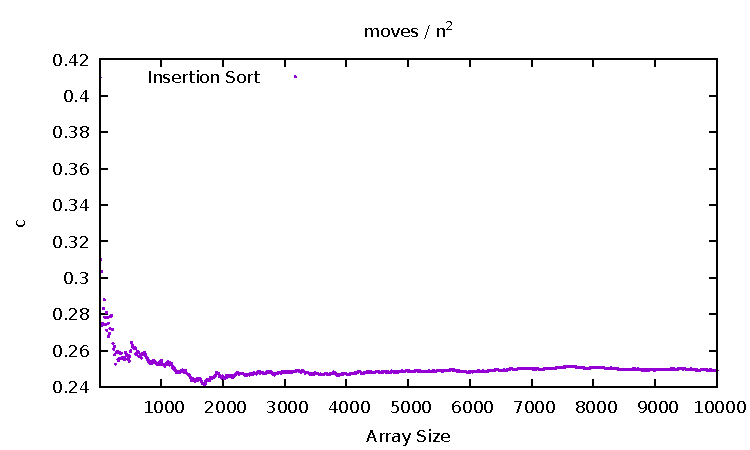
\includegraphics{plots/nn-moves-insertion.pdf}\caption{The ratio of moves to $x^2$ in Insertion Sort}
\end{centering}\end{figure}
\begin{figure}[H]\begin{centering}
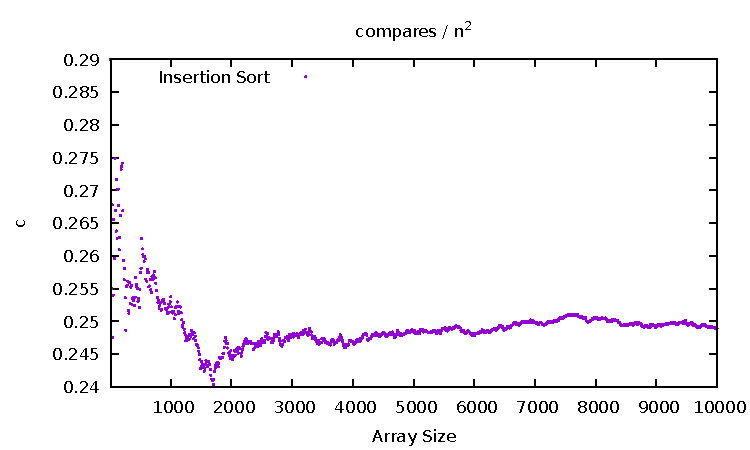
\includegraphics{plots/nn-compares-insertion.pdf}\caption{The ratio of compares to $x^2$ in Insertion Sort}
\end{centering}\end{figure}

\begin{figure}[H]\begin{centering}
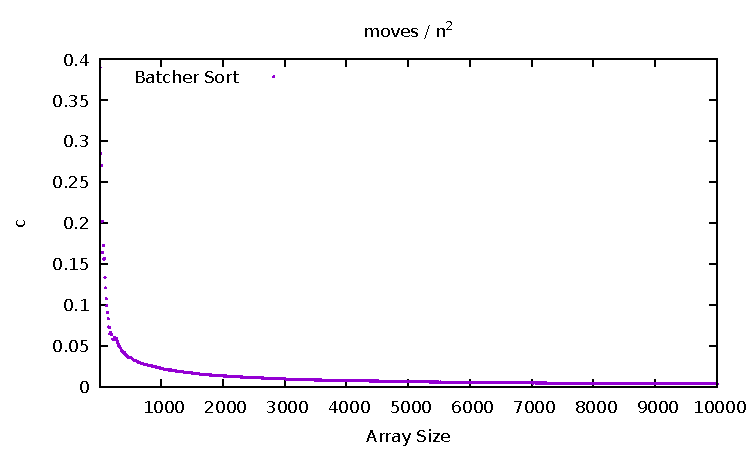
\includegraphics{plots/nn-moves-batcher.pdf}\caption{The ratio of moves to $x^2$ in Batcher Sort}
\end{centering}\end{figure}
\begin{figure}[H]\begin{centering}
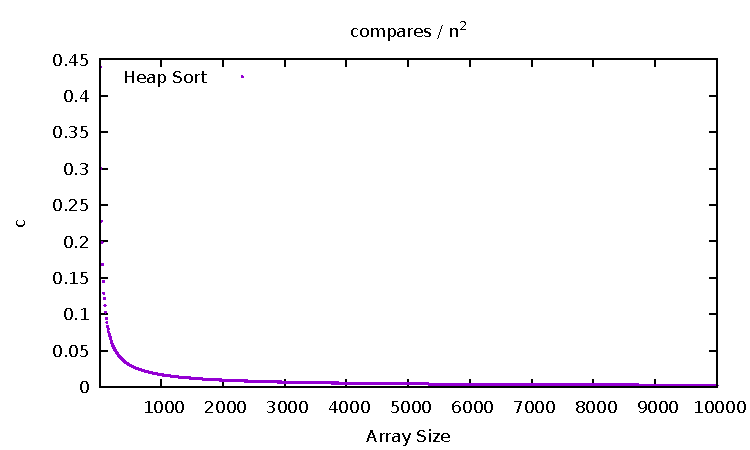
\includegraphics{plots/nn-compares-heap.pdf}\caption{The ratio of compares to $x^2$ in Heap Sort}
\end{centering}\end{figure}

\section{O Notation - Other Sorts}
However, when we graph the number of sorts and compares assuming $O(n\log(n))$ time, we get eye-opening results for the other three sorts. Graphing the number of sorts and compares over $n\log(n)$ provides almost constant results for all three sorts, each with their own quirks. Looking at the Batcher Sort graphs, we can see that the quotient increases over time. We can see that the derived constant $c \approx 2$ at $x = 100$. At $x = 1,000$, $c \approx 3$, at $x = 10,000$, $c \approx 4$, and so on. This shows that the $c$ ``constant" is not so constant with the Batcher Sort; in fact, it is relative to the number of elements: $c \approx \log_{10}(x)$. To be honest, I am not sure exactly \textit{why} it does that - I assumed the value would be proportional to the $\log_2(x)$, not $10$ of all numbers. Another interesting property of the Batcher Sort is the $c$ in the graph of comparisons - there are slight dips in the number of compares at each $x = 2^n$, where $n$ is an integer. This is because the sort works best with powers of two, so it will be relatively optimized at those points where it doesn't need to fill in any extra elements to recreate that behavior.

\begin{figure}[H]\begin{centering}
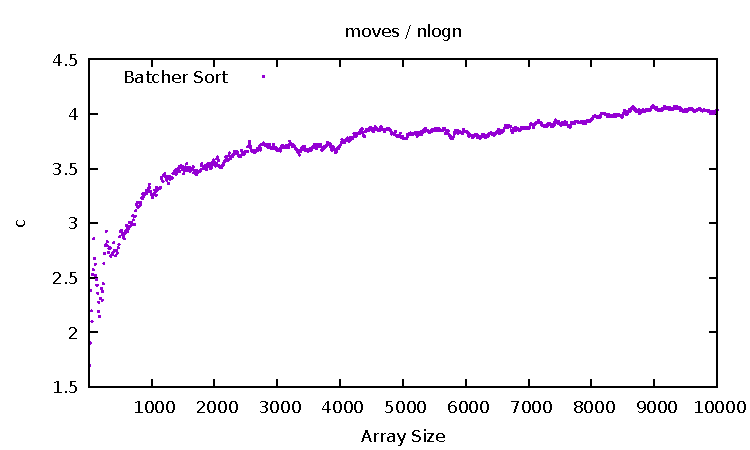
\includegraphics{plots/nlogn-moves-batcher.pdf}\caption{The ratio of moves to $x\log(x)$ in Batcher Sort}
\end{centering}\end{figure}
\begin{figure}[H]\begin{centering}
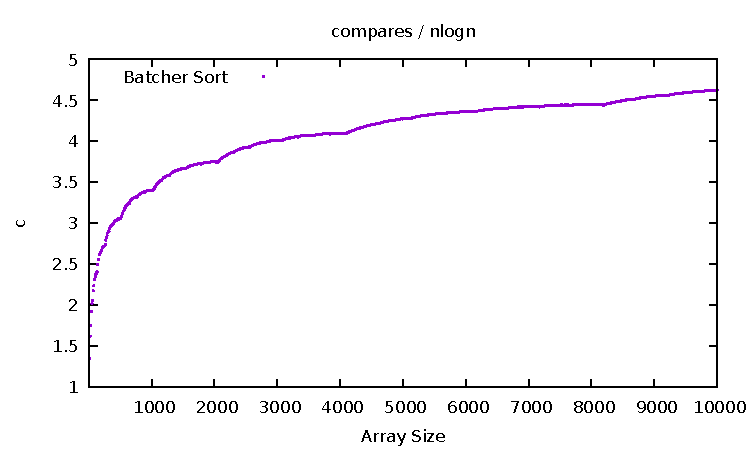
\includegraphics{plots/nlogn-compares-batcher.pdf}\caption{The ratio of compares to $x\log(x)$ in Batcher Sort}
\end{centering}\end{figure}

The Heap Sort graphs look sort of as expected - the $c$ constant averages out to $4$ and $2.5$ for the moves and compares, respectively. The difference in the $c$ constant between the Insertion Sort and these sorts explains why Insertion Sort is semi-competent at very small values - the constant overpowers the O notation.

\begin{figure}[H]\begin{centering}
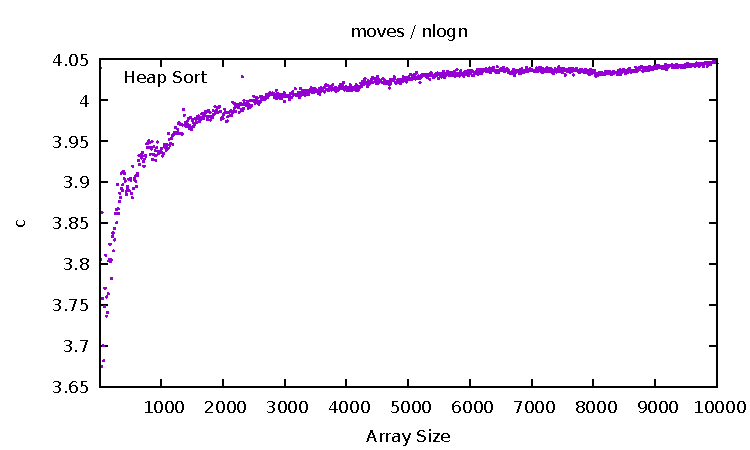
\includegraphics{plots/nlogn-moves-heap.pdf}\caption{The ratio of moves to $x\log(x)$ in Heap Sort}
\end{centering}\end{figure}
\begin{figure}[H]\begin{centering}
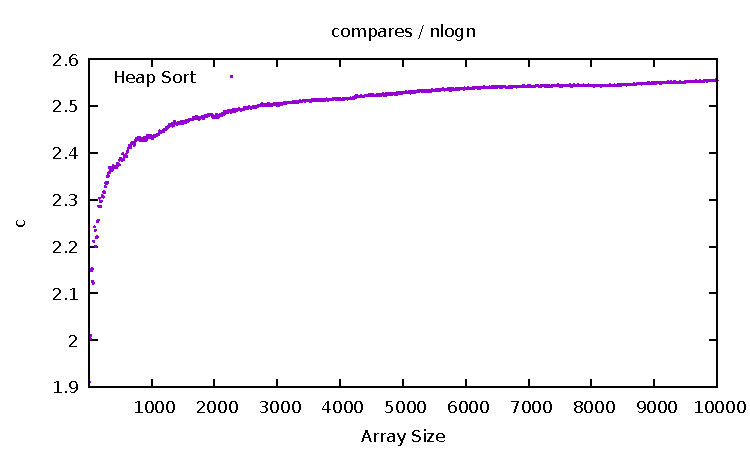
\includegraphics{plots/nlogn-compares-heap.pdf}\caption{The ratio of compares to $x\log(x)$ in Heap Sort}
\end{centering}\end{figure}

Quick Sort creates some spectacular graphs of moves and compares: the points are all over the place, though they stay at pretty consistent averages ($\approx 2.7$ and $1.6$). This is caused by Quick Sort's unstable algorithm as reflected in the jaggedness of the first two graphs: the efficiency jumps between $O(n\log(n))$ and $O(n^2)$. The fact that the $c$ constants are so low compared to Batcher and Heap sort indicates that Quick Sort is the most efficient of the three, which is confirmed by the first graphs comparing all the algorithms.

\begin{figure}[H]\begin{centering}
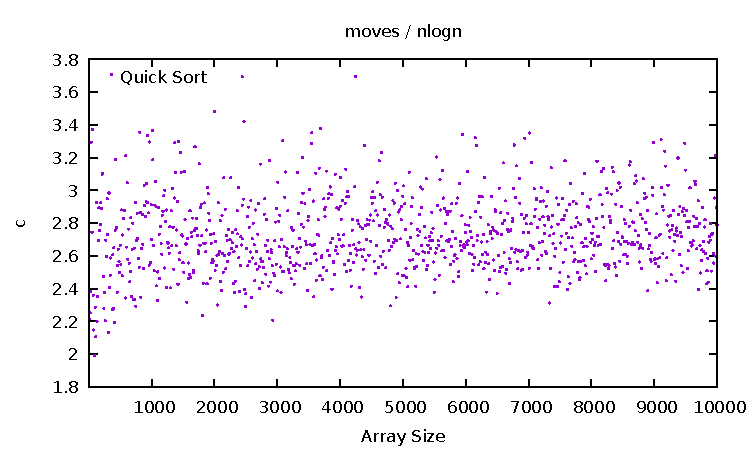
\includegraphics{plots/nlogn-moves-quick.pdf}\caption{The ratio of moves to $x\log(x)$ in Quick Sort}
\end{centering}\end{figure}
\begin{figure}[H]\begin{centering}
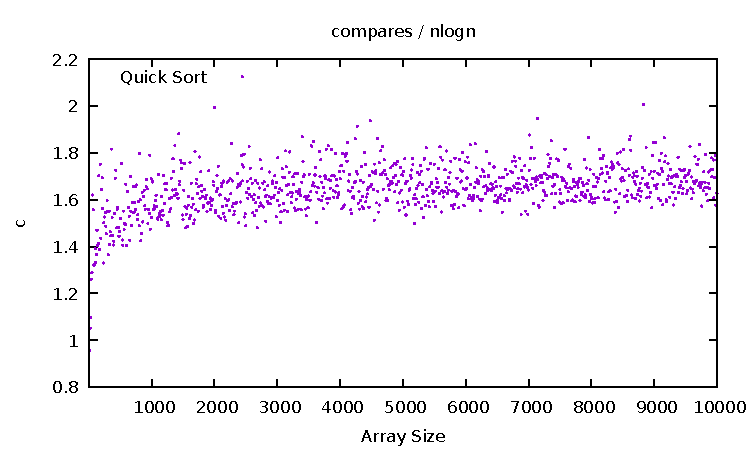
\includegraphics{plots/nlogn-compares-quick.pdf}\caption{The ratio of compares to $x\log(x)$ in Quick Sort}
\end{centering}\end{figure}

\section{Conclusion}
This assignment allowed a dive into some of the many possible sorting algorithms. It also highlighted the differences in algorithm efficiency, O notation, and how important the notation is when the input gets huge. Despite the speed of computers today, it is still extremely important to have optimized algorithms to calculate the result quickly and correctly. I also got insight into the $c$ constant in the O notation and its quirks: how it increases slowly in Batcher Sort, the effect it has on the efficiency of the algorithms at different scales, and the role it plays in trends. Lesson learned: work smarter, not harder.
\end{document}
